% !TeX root = ../../../wyrd.tex

\begin{WyrdSettingHeading}
    \WyrdCapLine{L}{ondon}, 1896. A city of gaslit streets, towering factories, and secrets lurking in the shadows. This is an era of progress, where steam and steel reshape the world—but beneath the veneer of industry and refinement, the old mysteries remain. The line between science and the supernatural is thinner than most would dare to believe.

    You are part of The Grand Society of Inquiry, a\\ prestigious organisation of detectives, scholars, and unconventional thinkers dedicated to unravelling the mysteries the world would rather forget. The police may handle mundane crimes, but when a case is impossible, when the authorities turn a blind eye, or when the answers defy reason, that is where you come in.

    The aristocracy hides more than it reveals. The city's underworld knows whispers of truths the elite wish to bury. Strange happenings unfold in laboratories, occult circles, and long-forgotten ruins. It is your job to investigate, to bring truth to light—whether the world is ready for it or not.

    You will encounter murderers whose motives defy logic, inventions beyond their time, secret societies vying for power, and horrors that exist just beyond the veil of reason. Some mysteries should never be solved—but you have chosen to chase the truth regardless.

    London may not thank you for what you uncover. The truth is rarely comforting. But if not you, then who?

    So, tell me: What mystery has found its way to your doorstep tonight?
\end{WyrdSettingHeading}

\section{Introduction}

\textit{The Grand Casebook} is both a setting and a toolkit for running episodic investigations in a world of steam-powered wonders, occult secrets, and unsolved mysteries. Set in a fictionalised London in the year 1896, the stories told here blend elements of classic detective fiction, gothic horror, and speculative science. At the heart of it all is the Grand Society of Inquiry, a secretive organisation dedicated to uncovering truths that others fear to face.

This chapter serves as a guide for running stories in this world. Within, you'll find an overview of the setting, key factions, and recurring threats. It offers guidance for players creating characters within this shared universe, and for GMs constructing compelling mysteries. Each scenario is self-contained, making it ideal for one-shots or rotating player groups—but taken together, the cases reveal a wider world of intrigue, danger, and creeping dread.

\newcolumn
\noindent Expect:
\begin{itemize}\raggedright
    \item Rich, gaslit atmosphere full of secrets and contradictions
    \item Investigations that challenge reason and morality
    \item Encounters with both human depravity and supernatural horror
    \item A flexible structure that supports drop-in/drop-out episodic play
\end{itemize}

\vspace{.75\baselineskip}\noindent
Whether you’re a veteran investigator or a newcomer to the shadows, this chapter provides all the tools you need to begin your journey into London’s most perilous enigmas.


\section[The World of the Grand Casebook]{The World of the\\ Grand Casebook}

London in 1896 is a city of contradictions. At its heart lies a tension between progress and tradition, the rational and the arcane. Airships drift over soot-covered rooftops, automata assist in the factories, and steam-powered cabs rattle through cobbled streets. Yet for all these marvels of industry, old fears still linger in the fog. Ancient horrors persist in forgotten crypts, and whispers of the occult echo in gentlemen’s clubs and back-alley gatherings.

This is a world where gaslight barely holds back the darkness, where rational minds struggle to explain the inexplicable. The Grand Casebook embraces the interplay between Victorian-era crime fiction, steampunk ingenuity, and gothic supernatural horror.

\vspace*{\fill}
\begin{center}
    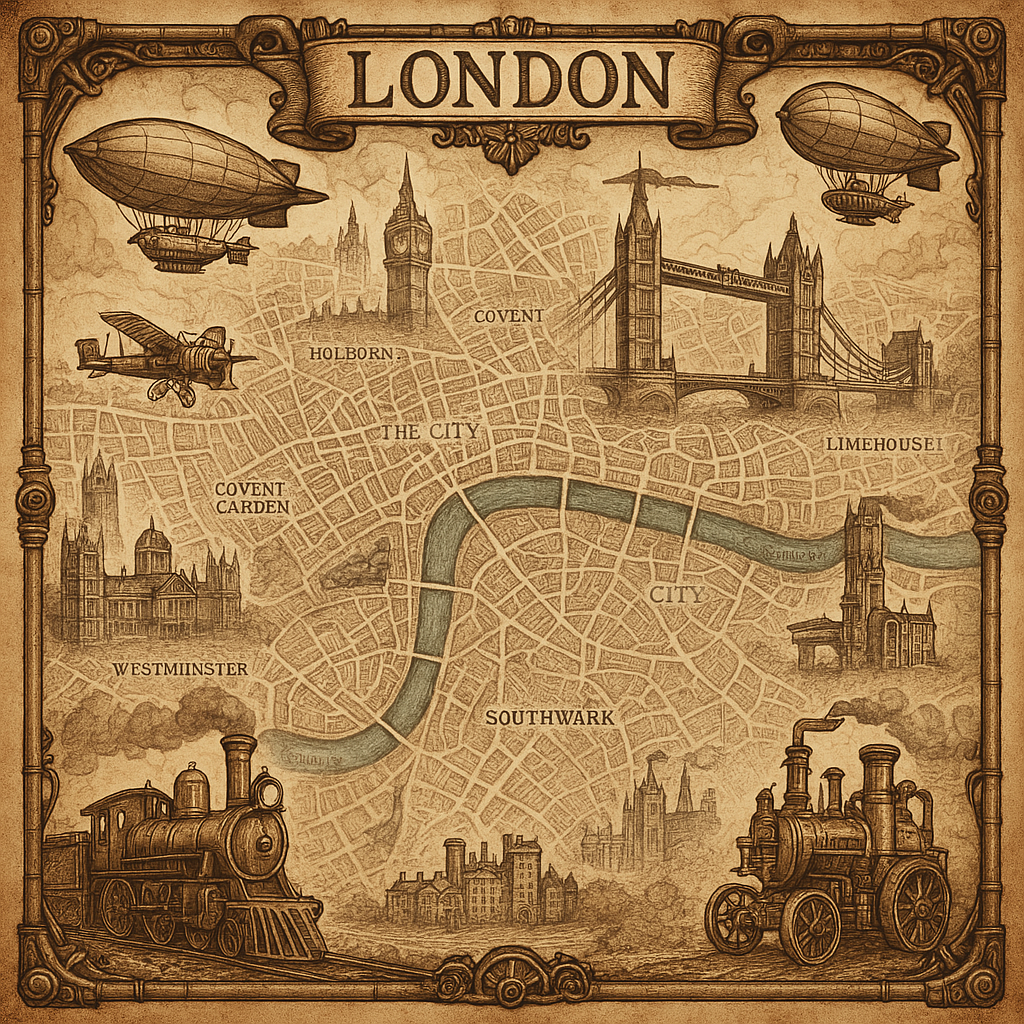
\includegraphics[width=\linewidth]{img/pageart/london-map}
\end{center}
\vspace*{\fill}


\subsection{Technology and Magic}

London in 1896 stands at the precipice of modernity. Steam-powered inventions, mechanical marvels, and new sciences have transformed daily life for many of the city's citizens. Airships cross the Thames, pneumatic tubes shuttle messages through walls, and automata clatter away in factories and households alike. The line between miracle and machine is increasingly blurred, and the pace of progress shows no signs of slowing.

Yet beneath this veneer of industrial achievement lies something older—and far stranger.

Technology in the world of \textit{The Grand Casebook} is advanced, but not unbounded. Engineers and inventors push beyond the limits of Victorian science, crafting devices that seem miraculous yet remain grounded in gears, steam, and brass logic. Devices such as:
\begin{itemize}
    \item Aetheric resonators that detect unseen energies
    \item Self-writing pens linked to voice-capturing cylinders
    \item Automatons that can mimic human speech and movement (and might be getting sentient)
    \item Steam-powered prosthetics with semi-autonomous reflexes
    \item Clockwork spiders used for surveillance and sabotage
\end{itemize}
While the upper classes marvel at these wonders, many working-class Londoners view them with suspicion or unease.

Magic, on the other hand, is not publicly\\ acknowledged. It exists in the margins—rumours whispered in taverns, symbols etched into cellar doors, or strange phenomena dismissed as mass delusion. Most Londoners scoff at the idea of the supernatural, even as they shudder when crossing graveyards alone or burn sage to ward off nightmares.

Occult knowledge is rare and often dangerous. Practitioners speak of ley lines, dream-keys, and veiled realities that slip through cracks in the waking world. True magic is subtle, costly, and often maddening. Examples might include:
\begin{itemize}
    \item A mesmerist who can force confessions through whispered suggestion
    \item A cursed mirror that reflects a different version of the past
    \item Blood-ink sigils that reveal invisible messages only at dusk
    \item Seances that summon not the dead—but something wearing their voice
\end{itemize}

The \textbf{Grand Society of Inquiry} stands at the intersection of these forces. Some members pursue strange sciences; others study grimoires or collect arcane relics. Most tread cautiously, for they know too well that the boundary between invention and invocation is perilously thin.

\textit{In this world, truth wears a mechanical face and a hidden name—and it is up to the investigators to uncover both.}

\subsection{The Grand Society of Inquiry}

The Grand Society of Inquiry was founded in the aftermath of the Crimean War. It emerged from a coalition of scholars, detectives, and adventurers who recognised that some mysteries lay beyond the reach of conventional authorities.

Though their official purpose is to investigate “unusual” occurrences, they function as much as a secret society as they do an investigative agency. Its members hail from all walks of life—former police officers, rogue academics, disgraced aristocrats, and those who have glimpsed the supernatural and can never return to ignorance.

The Society operates in secrecy, liaising with those who possess forbidden knowledge—whether they be alchemists, mesmerists, or reformed criminals. Their headquarters, a sprawling archive hidden beneath a London bookshop, contains a vast trove of esoteric knowledge accessible only to a select few.

\subsection{The Powers That Be}

While the Society pursues truth, others work to obscure it. Various factions hold sway over London, each with their own interest in the city’s secrets:

\begin{itemize}\raggedright
    \item \textbf{Scotland Yard:} The official enforcers of law and order. Most officers dismiss the supernatural, though a handful of seasoned inspectors know better. The Yard tolerates the Society only when their interests align.
    
    \item \textbf{The Ministry of Esoteric Affairs:} A clandestine government branch tasked with monitoring supernatural activity. Their agents operate with impunity, and their motives often clash with the Society’s.
    
    \item \textbf{The Order of the Silver Dawn:} An occultist cabal that seeks power through ritual and ancient knowledge. Some whisper their origins stretch back to the Elizabethan court.
    
    \item \textbf{The Industrial Magnates:} The city’s great industrialists have secrets of their own—from illicit experiments to pacts with entities beyond comprehension.

    \item \textbf{The Aetheric Liberty Assembly:} A group of scientists, inventors and philosophers who believe that automata are gaining sentience and should be treated as equals. They advocate for the rights of machines and seek to liberate them from their servitude.
    
    \item \textbf{The Automata Liberation Army:} A radical faction of the Aetheric Liberty Assembly willing to go to any length to achieve freedom and independence for thinking machines.
    
    \item \textbf{The Underworld Syndicates:} Smugglers and thieves have always known that London’s alleys and docks are haunted by more than mere criminals.
\end{itemize}

Use the powerful fractions in the setting to create tension and conflict that can span over multiple games without substantially changing the situations for the player characters. This way, the players can feel the weight of the world around them, and their actions can have consequences, but it is still possible for players to sit out without needing to worry about missing out on the story.

The players may find themselves caught in the crossfire of these factions, each with their own agendas and goals. The Society may ally with one faction against another, or they may find themselves at odds with all of them.



\section[Playing in the Grand Casebook]{Playing in the\\ Grand Casebook}

The Grand Casebook is structured as an episodic, mystery-driven setting. Each session presents a new case to unravel, though overarching plots may weave between episodes. Every game is designed as a standalone investigation, with varying player characters and threats. Types of mysteries include:

\begin{itemize}
    \item \textbf{Classic Crime:} Murders, thefts, and conspiracies with unexpected twists.
    \item \textbf{Scientific Anomalies:} Rogue automata, unstable inventions, or experiments gone awry.
    \item \textbf{Supernatural Encounters:} Hauntings, curses, and otherworldly horrors.
    \item \textbf{Political Intrigue:} Blackmail, espionage, and aristocratic conspiracies.
    \item \textbf{Exploratory Adventures:} Forgotten asylums, hidden laboratories, and haunted ruins.
\end{itemize}

\subsection{Character Roles}

Players take on the roles of Society agents, each bringing unique skills and perspectives to the investigative team. Sample archetypes include:

\begin{itemize}\raggedright
    \item \textbf{The Detective:} A seasoned investigator with a sharp mind and keen eye for detail.
    \item \textbf{The Scientist:} A genius innovator whose inventions often outpace their safety.
    \item \textbf{The Occultist:} A scholar of forbidden knowledge, versed in ritual and arcane lore.
    \item \textbf{The Rogue:} A streetwise scoundrel with contacts in the city’s underworld.
    \item \textbf{The Aristocrat:} A socialite with access to influential circles and hidden secrets.
    \item \textbf{The Soldier:} A hardened veteran, able to face danger head-on.
\end{itemize}

\subsection{Creating Connections}

Though each case in \textit{The Grand Casebook} may\\ introduce a different roster of investigators, shared history and interpersonal ties enrich the narrative and help players engage more deeply with one another. These connections don't need to be\\ elaborate—they might stem from a single case, a whispered rumour, or a common enemy.

Here are a few ways to establish meaningful links between characters:

\begin{itemize}\raggedright
    \item \textbf{Shared Cases:} The investigators have worked together before. Perhaps one covered for the other's mistake, or they both saw something they swore never to speak of again.
    
    \item \textbf{Mentorships and Rivalries:} One character may have trained another, or they may have taken opposing stances in a past inquiry. Old rivalries can add drama to even the most routine investigation.
    
    \item \textbf{Family or Academic Ties:} Some investigators may be siblings, cousins, or former colleagues at a university or academy—connected by blood, scandal, or shared disgrace.
    
    \item \textbf{Secrets and Debts:} One character knows something the other must keep hidden. Or perhaps a favour was granted years ago—and the time has come to repay it.
    
    \item \textbf{Unfinished Business:} A case from the past remains unresolved, and its shadow looms over the current investigation. What went wrong, and who bears the blame?
\end{itemize}

To help generate quick connections, consider the following sample bonds:

\begin{itemize}\raggedright
    \item \textit{“You were the only witness to what I saw that night—and you promised to never speak of it.”}
    \item \textit{“We once faced something inhuman together. We haven’t spoken since.”}
    \item \textit{“I saved your life in a fire. You’ve never asked how I knew to be there.”}
    \item \textit{“We both tried to warn them, and they laughed. Now the laughter has stopped.”}
    \item \textit{“You were meant to take the case. I took it instead, and someone died.”}
\end{itemize}

Players are encouraged to create new bonds at the beginning of each session or case. Even if characters change from one mystery to the next, those connections ensure that each team feels like part of a larger web—a living archive of shared secrets, triumphs, and regrets.

\subsection{Setting Rules}

The Grand Casebook modifies standard play to reflect its distinctive tone. Consider the following adjustments:

\begin{itemize}\raggedright
    \item \textbf{Stress:} Psychological stress plays a prominent role, with lingering trauma from particularly harrowing encounters. In less action-heavy scenarios, fatigue and wounds may be omitted entirely in favour of roleplay.
    
    \item \textbf{Tools of the Trade:} Players may use unique investigative gadgets such as aetheric spectrometers, spirit lenses, or sonic decoding rods.
    
    \item \textbf{Mystery Structure:} Adventures focus on gathering evidence, piecing together clues, confronting suspects, and unveiling the truth—sometimes at a cost.
    
    \item \textbf{Supernatural Threats:} Some threats cannot be overcome by force alone and require specific rituals, research, or cunning to defeat.
\end{itemize}

\subsection{Example Skill List}

A non-exhaustive list of skills is provided below. These skills are designed to be broad and flexible, allowing players to adapt them to their characters' backgrounds and the specific challenges they face. The Grand Casebook setting does not use detailed skills as the types of scenarios are more mystery focused and do not require a large number of skill rolls. Feel free to modify or expand upon this list as needed.

\subsubsection*{Investigation \& Knowledge}  
\begin{itemize}\raggedright
    \item \emph{Investigate}---Analysing crime scenes, following leads, searching for hidden clues.
    \item \emph{Lore}---Understanding history, science, the occult, and the unnatural.
    \item \emph{Notice}---Spotting details, sensing danger, and staying aware of surroundings.
\end{itemize}

\subsubsection*{Social \& Influence}  
\begin{itemize}\raggedright
    \item \emph{Rapport}---Gaining trust, persuading, and negotiating.
    \item \emph{Deceive}---Lying, creating convincing cover stories, and disguises.
    \item \emph{Provoke}---Intimidation, interrogation, and getting a reaction from others.
    \item \emph{Contacts}---Knowing the right people and gathering information through connections.
    \item \emph{Empathy}---Reading emotions, understanding motives, and connecting with others.
\end{itemize}

\subsubsection*{Physical \& Dexterity}  
\begin{itemize}\raggedright
    \item \emph{Athletics}---Running, jumping, climbing, and escaping dangerous situations.
    \item \emph{Stealth}---Moving unseen, tailing a suspect, sneaking into restricted areas.
    \item \emph{Fight}---Engaging in hand-to-hand combat, fencing, or using melee weapons.
    \item \emph{Shoot}---Firearms, throwing weapons, and ranged combat.
\end{itemize}

\subsubsection*{Resilience \& Willpower}
\begin{itemize}\raggedright
    \item \emph{Will}---Resisting fear, staying composed under pressure, enduring mental strain.
    \item \emph{Physique}---Strength, endurance, and the ability to withstand injury or exhaustion.
\end{itemize}

\subsubsection*{Mechanical \& Practical Skills}  
\begin{itemize}\raggedright
    \item \emph{Burglary}---Lockpicking, safecracking, and breaking into places unseen.
    \item \emph{Resources}---Access to wealth, favours, or valuable possessions.
    \item \emph{Crafts}---Repairing devices, modifying tools, or working with mechanical systems.
\end{itemize}

\subsection{Example Traits and Gear}

Traits can be used to tie a character to the setting and to give them a unique flavour. Feel free to add traits that include elements of steampunk or the supernatural, but otherwise center them on the investigation theme of the setting.

\begin{itemize}\raggedright
  \item \textbf{Master of Disguise} — You may create disguises quickly and convincingly, gaining a bonus when impersonating others or blending into unfamiliar crowds.
  \item \textbf{Whispers from Beyond} — You occasionally receive cryptic insight from unseen forces. Once per session, ask the GM a yes/no question and get a truthful answer.
  \item \textbf{Clockwork Reflexes} — Whether through training or augmentation, your reaction time is uncanny. Gain a bonus when acting on initiative or avoiding traps.
  \item \textbf{Read Like a Book} — You can pick up a person’s emotional state and intentions at a glance. Gain a bonus when using empathy or social observation.
  \item \textbf{Unflappable} — You remain calm even under supernatural stress or mortal peril. Gain a bonus when resisting fear or deception.
  \item \textbf{Ironclad Logic} — Your deductions are rigorous and methodical. Once per session, declare a clue’s correct interpretation—even if misdirected evidence says otherwise.
  \item \textbf{Heir to Secrets} — You’ve inherited knowledge most would call heretical. Gain narrative permission to recognise occult symbols, forbidden tomes, or cursed artefacts.
\end{itemize}

\vspace{.75\baselineskip}
\noindent Gear can include signature equipment, tools, or steampunk devices that provide unique capabilities. 

\begin{itemize}\raggedright
  \item \textbf{Investigator’s Satchel}  
  \begin{itemize}
    \item \emph{Trait: Everything Has Its Place} — Gain a bonus when producing a needed item from your well-stocked kit, especially during investigations or field work.
  \end{itemize}
  
  \item \textbf{Phlogiston Lantern}  
  \begin{itemize}
    \item \emph{Trait: Reveals the Unseen} — This experimental lantern emits spectral light, revealing hidden markings, footprints, or magical residue in darkened places.
  \end{itemize}

  \item \textbf{Pneumatic Communicator Badge}  
  \begin{itemize}
    \item \emph{Trait: Whisper on the Wire} — Allows secure short-range communication between members of the Society. Gain narrative permission to call for backup or coordinate plans.
  \end{itemize}

  \item \textbf{Electro-Prod Gauntlet}  
  \begin{itemize}
    \item \emph{Trait: Shock and Awe} — This weaponized glove can deliver a non-lethal shock. Gain a bonus when subduing an opponent in close quarters.
  \end{itemize}

  \item \textbf{Monocle of Magnification}  
  \begin{itemize}
    \item \emph{Trait: Forensic Precision} — Gain a bonus when examining fine details or spotting what others miss at a crime scene.
  \end{itemize}
\end{itemize}



\subsection{Running the Casebook}

\noindent
\textit{The Grand Casebook} is designed for episodic, mystery-driven play. Each scenario presents a self-contained case that can be resolved within a single session, though connections between investigations may form a broader narrative arc. Whether you're running a one-shot or a full campaign, the goal is to deliver tense, atmospheric stories that blend deduction, drama, and the uncanny.

\subsubsection*{Tone and Style}

Mysteries in this setting walk the line between gothic horror and rational inquiry. While some cases may seem purely mundane at first glance, others hint at deeper, more unsettling truths. Even when a case has a supernatural core, the horror should feel restrained and eerie rather than overtly fantastical.

Embrace the unknown. Some truths are best left in shadow—half-glimpsed, half-understood. Let the players gather fragments, whispers, and echoes. In the end, it should be their choice to believe they’ve unraveled the mystery… or merely kept its tendrils at bay.


\subsubsection*{Structure of a Case}

Most scenarios follow a common rhythm:

\begin{enumerate}
    \item \textbf{The Hook:} A murder, anomaly, or strange event draws the investigators in.
    \item \textbf{Initial Clues:} Clues and NPCs point in several possible directions. Dead ends, red herrings, and cryptic statements build tension.
    \item \textbf{The Descent:} As the truth emerges, the tone shifts. Strange phenomena escalate. Players must make difficult choices.
    \item \textbf{The Confrontation:} The truth is revealed or confronted. It may be stopped, understood, or escaped—but not always cleanly.
    \item \textbf{Aftermath:} Each case leaves ripples—on the world, on the characters, and on the unseen forces watching from beyond.
\end{enumerate}

\begin{CommentBox}{Episodic Play and Continuity}
    Each case is self-contained, but recurring characters, unresolved threads, and subtle callbacks help create a richer world. Let players choose how much continuity they want—some groups may prefer standalone cases, while others enjoy a growing conspiracy in the shadows.
\end{CommentBox}

\subsubsection*{Pacing and Player Choice}

Don’t railroad players toward a single solution. Instead, present a web of clues and allow the group to connect them in their own way. Keep scenes focused—each should either reveal something, raise a question, or increase tension. Let the story breathe between moments of revelation and danger.

Use quick NPC sketches, recurring motifs (a black carriage, an out-of-place clock, a phrase that recurs), and sensory detail to evoke the setting.

\subsubsection*{Consequences Matter}

This setting thrives on ambiguity and moral tension. Solving a case may not mean saving everyone. Sometimes the wrong person goes free. Sometimes knowing the truth is worse than ignorance. Let the players’ decisions shape future cases, and don’t be afraid to revisit old threads in unexpected ways.

\subsubsection*{Mixing Horror and Mystery}

Mystery is about uncovering what’s hidden. Horror is about what should remain hidden. When blended, these genres create a powerful effect: the sense that knowing too much carries its own price. Use this interplay to your advantage. Offer tantalising truths—but ensure some doors are better left closed.


\subimport{./}{npcs}
\subimport{./}{player-characters}
\subimport{./}{case-files}